%\usepackage{amsmath}
%\usepackage{hyperref}
%\usepackage{amsthm}
%\usepackage{graphicx}
\documentclass[journal, a4paper]{IEEEtran}
\usepackage[italian]{babel}
\usepackage{booktabs}
\usepackage{siunitx}%Questo serve a caricare il pacchetto delle unità di misura del sistema internazionale%
\usepackage[utf8]{inputenc}
\usepackage{graphicx} 
\usepackage{url}
\usepackage{amsmath}
\usepackage{amssymb}


\usepackage{keyval}
\usepackage{xcolor}
\usepackage{caption}
\usepackage{tikz}
\usepackage{circuitikz}
\usepackage{authblk}
%\usepackage{hyperref}

\begin{document}


% Define document title and author
	\title{Tecnologie Digitali - Logbook Week 5}
	\author[1]{Salvatore Bottaro}
		\author[2]{Lorenzo M. Perrone}
		\affil[1]{\texttt{salvo.bottaro@hotmail.it}}
		\affil[2]{\texttt{lorenzo.perrone.lmp@gmail.com}}
	\markboth{Tecnologie Digitali - Di Lieto}{}
	\maketitle
	
\begin{abstract}
	Logbook di laboratorio di Tecnologie Digitali, a.a. 2015/2016. Week 5.
\end{abstract}

\section{Meccanismo e caratteristica I-V del LED}
In un LED il meccanismo di emissione della luce avviene in seguito ad un processo di ricombinazione fra le cariche presenti nella banda di conduzione e quelle nella banda di valenza. Il processo porta all'emissione di un fotone di energia:
\begin{equation}
\Delta E = h \, \frac{c}{\lambda}
\end{equation}

Dal momento che $hc$ = 1240 eV $\cdot$ nm, questo suggerisce una regola mnemonica per convertire in eV le lunghezze d'onda espresse in nm:

\begin{equation}
\Delta E = \frac{1240}{\lambda(nm)} \; eV
\end{equation}

Ad esempio nel caso di luce blu, $\lambda = 470$ nm, si ottiene $\Delta E \approx 2.6$ eV.\\
Per una prima stima della costante di Planck abbiamo impiegato un LED rosso (645 nm) modello HLMP-C115, realizzando sulla breadboard il circuito dello schema in figura \ref{fig:led_circ}.\\

\begin{figure}[htp]
\centering
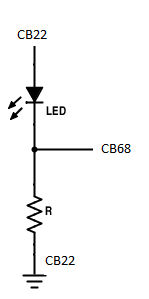
\includegraphics[scale=.6]{led_circ}
\caption{Schema del circuito realizzato sula breadboard. Sono indicate anche le porte della scheda di acquisizione impiegate.}
\label{fig:led_circ}
\end{figure}

Dal datasheet di HLMP-C115 è possibile leggere il massimo valore per la corrente diretta:
\begin{equation}
I_F = 30\, mA
\end{equation}

che pone un vincolo sul valore minimo della resistenza R. Questo può essere dedotto osservando la caratteristica I-V del LED riportata nel datasheet (figura \ref{fig:c115car}).

\begin{figure}[htp]
\centering
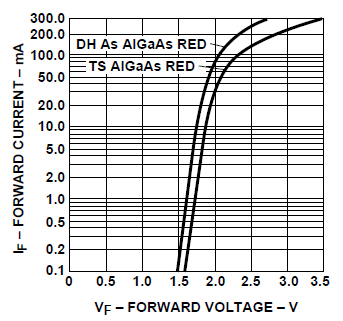
\includegraphics[scale=.6]{IF-VF}
\caption{Curva caratteristica del LED che si può leggere nel datasheet. Il modello da noi impiegato corrisponde al DH As AlGaAs RED.}
\label{fig:c115car}
\end{figure}

Come si vede se V è la tensione di ingresso, $\Delta$V la tensione diretta ai capi del LED in funzione della corrente I, si ha che R vale:
\begin{equation}
R = \frac{V-\Delta V}{I}
\end{equation}

Per V = 10 V (massima tensione generata dalla scheda), I = $I_F$, $\Delta$V $\approx$ 1.8 V (tensione diretta a cui la corrente che scorre nel LED è quella massima) si ottiene:
\begin{equation}
R_{min} \approx 275 \, \Omega
\end{equation}

Nell'esperienza abbiamo impiegato una resistenza R = 470 $\pm$ 0.8 $\%$. In queste condizioni è possibile stimare sempre dalla curva di figura \ref{fig:c115car} che applicando una tensione di ingresso da 10 V la corrente massima nel circuito risulti circa 18 mA. Infatti bisogna individuare il punto di intersezione fra la curva caratteristica del LED e la retta V = 10 V - R$\cdot$I, che si vede facilmente essere compreso in 1.5 V $\leq$ V $\leq$ 2 V e 1.7 mA $\leq$ I $\leq$ 1.8 mA.\\

Abbiamo infine montato il circuito di figura \ref{fig:led_circ} sulla breadboard. Con il VI \textbf{\texttt{Vin$\_$Vout$\_$2015}} abbiamo impostato diversi valori della tensione di ingresso, ricavando da $V_{out}$ il valore della corrente che scorreva nel LED. I valori misurati sono riportati in tabella \ref{tab:firstmis}.

\begin{table}[htp]
\centering
\caption{Prime misure della corrente nel LED. I valori di $V_{in}$ riportati sono quelli impostati nel VI.}
\label{tab:firstmis}
\begin{tabular}{|c|c|c|}
\hline 
$V_{in}$ (V)& $V_{out}$ (V)& I (mA)\\ 
\hline 
1 & 0 & 0 \\ 
\hline 
2 & 0.4053(7) & 0.862(7) \\ 
\hline 
3 & 1.3289(11) & 2.83(2) \\ 
\hline 
4 & 2.297(4) & 4.89(4) \\ 
\hline 
5 & 3.299(8) & 7.02(6) \\ 
\hline 
\end{tabular}
\end{table} 
 
Abbiamo poi effettuato delle misure impostando $V_{in}$ fra 1 V e 2 V, poiché si è visto che il LED si accende proprio in questo intervallo. Le misure effettuate sono riportate in tabella \ref{tab:secmis}.

\begin{table}[htp]
\centering
\caption{Determinazione della corrente di prima accensione del LED.}
\label{tab:secmis}
\begin{tabular}{|c|c|c|c|}
\hline 
$V_{in}$ (V)& $V_{out}$ (mV)& $V_{LED}$ (V) & I ($\mu$A)\\ 
\hline 
1.3 & 0 & 0 & 0 \\ 
\hline 
1.35 & 2.44(0) & 1.348 & 5.19(4) \\ 
\hline 
1.4 & 4.88(6) & 1.39 & 10.38(8) \\ 
\hline 
1.5 & 22.1(4) & 1.4779 & 47.0(4) \\ 
\hline 
\end{tabular} 
\end{table} 
 
In particolare abbiamo individuato il punto di prima accensione del LED per $V_{in}$ = 1.35 V, cui corrisponde una \textit{forward voltage} $V_f$ = 1.348(BOH) e una corrente $I_f$ = 5.19(4) $\mu$A. Per quanto riguarda l'errore riportato per alcuni valori di $V_{out}$, il fatto che in qualche caso si sia riportato 0 è dovuto al fatto che l'errore calcolato dal VI \textbf{\texttt{Vin$\_$Vout$\_$2015}}, ovvero la deviazione standard su un certo numero di misure, era più piccolo del minimo valore riportabile. Eseguendo infatti la stessa misura con \textbf{\texttt{Traccia$\_$Vin$\_$Vout}} nelle stesse condizioni con fondoscala 0.05 V, i punti ottenuti avevano la stessa ordinata a parte 2 punti che differivano dagli altri di COME SI CHIAMA?

\subsection{Stima di \textit{h}} 
Tramite il VI \textbf{\texttt{Traccia$\_$Vin$\_$Vout}} abbiamo campionato l'equivalente della caratteristica I-V del LED. Infatti come si vede in figura \ref{fig:ledcar}, si è misurata la tensione $V_{out}$ in funzione di $V_{in}$, da cui ovviamente è possibile risalire alla corrente che scorre nel LED semplicemente dividendo per la resistenza R. \\

\begin{figure}[htp]
\centering
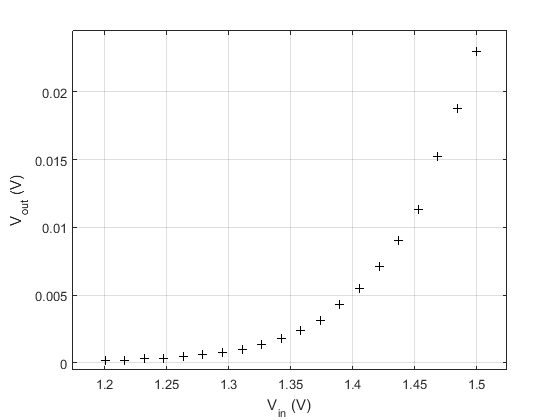
\includegraphics[scale=.6]{graph_led}
\caption{Grafico dei dati sperimentali di $V_{out}$ in funzione di $V_{in}$ equivalente alla caratteristica I-V.}
\label{fig:ledcar}
\end{figure}

Dal grafico si vede come la corrente comincia a crescere rapidamente per $V_{out}$ = 1.37 V $\pm$ 0.02 V, compatibile con il valore trovato per la tensione di prima accensione del LED, e che può essere presa come stima della $V_{gap}$ fra la banda di conduzione e di valenza. Da qui, tramite:
\begin{equation}
h = \frac{\lambda e V_{gap}}{c}
\end{equation}

è possibile fornire una prima stima di h. Utilizzando i valori di \textit{e} e \textit{c} universalmente accettati forniti da \texttt{CODATA}:
\begin{equation}
e = 1.6021766208(98) \cdot 10^{-19} \, C
\end{equation}
\begin{equation}
c = 299 792 458 \, \frac{m}{s}
\end{equation}

mentre come valore della lunghezza d'onda emessa dal diodo abbiamo preso $\lambda$ = 645 nm $\pm$ 12 nm, ovvero il valore di picco e come errore la HWHM che si può dedurre dal grafico dell'intensità relativa in funzione della lunghezza d'onda che si trova nel datasheet. Si ottiene così:
\begin{equation}
h_{ext} = (4.7 \pm 0.2) \cdot 10^{-34} Js
\end{equation}

Come si può notare, il valore stimato differisce di circa il 30 $\%$ da quello attualmente accettato. Difatti il metodo impiegato si basa su una scelta soggettiva del valore di soglia per la stima di $V_{gap}$ nella caratteristica I-V del LED. Tuttavia nonostante ciò la stima è ragionevole.

\end{document}